\section{The Reason Why the Same Results Do Not Happen at Twelve-Year Intervals. Why Bad Results Happen Although Good Were Expected and Vice-Versa. Why Great Good or Bad Results Happen Even Though the Distribution is Located in Empty Signs (9K,6P)}

It is necessary to inspect the past, the current, and the future chronocrators and to determine if they are passing from propitious \textbf{/219K/} to impropitious, or from malefic to benefic places. <I say this> because often a nativity experiences an anxious period subject to the law and is condemned because of the
chronocratorship of malefics. Later, however, when benefics take over and when the overall chronocratorship indicate that the nativity is secure, the nativity experiences a restoration of rank and livelihood
through some defenses and the basis of the nativity advances to greater fortune. But whenever the nativity is carried to an inferior overall chronocratorship, and the chronocrators are in accord, then various disputes, accusations, trials, losses, and hatreds are prepared in advance until the nativity meets the crisis which is fated to happen. 
In the same way, if a cause of good occurs in the sequence of chronocrators, then friendships, associations and ties with the great, stewardships, legacies, and gifts are prepared.

As a result, those who were lowly and weak in their period of crisis are treated as noble, sensible, and charming because of the terms of good fortune. On the other hand, \textbf{/209P/} those who are entirely
courageous and well educated (at least, according to the basis of the nativity from the beginning) are condemned and are considered coarse, cowardly, and ineffective, and they are oppressed by their inferiors. These men bear their abasement nobly and yield to the laws of Fate. 

In the case of ruling nativities, we find that when the chronocrators are making the transition in succession with the others, even though the time of rule has not yet been reached, some men attain noteworthy and profitable rank, others tarry in an opposite, ruinous condition. As a result, for some men bad things become good and a source of safety; for others even apparent good later becomes a cause of evil.

Fate has decreed for each person the immutable working out of events, reinforcing this decree with many opportunities for good or bad consequences. Through the use of these opportunities, two self begotten gods, Hope and Fortune, the assistants of Fate, control man’s life and make it possible for him to bear Fate’s decrees by using their compulsion and deception. One of the two <Fortune> manifests herself to everyone through the forecasted outcome, proving herself to be good and kind at one time, at another time dark and grim. Fortune raises some high only to cast them down, and degrades others only to raise them to glory. \textbf{/220K/} 

The other of the two <Hope> is neither dark nor bright; she moves everywhere in disguise and in secret, smiling on everyone like a flatterer, and she displays many attractive prospects which cannot be attained. She controls men by deceiving them: these men, even though they were wronged and were enslaved to their desires, still are attracted to her again, and full of Hope, believe that their wishes will be fulfilled. They believe her—only to get what they do not expect. If Hope ever does offer solid prospects to anyone, she immediately abandons him and goes on to others. She seems to be close to everyone, but she stays with no one. As a result, those ignorant of the prognostic art—or those not willing to engage in it at all—are led
away and enslaved to these previously mentioned gods. They endure all blows and suffer punishment along with their pleasures. Some partially attain what they hoped for, their confidence begins to increase, and they await a permanently favorable outcome—not realizing how precarious and slippery are these accidents of Fortune. Others are disappointed in their expectations not just once, but always; they then surrender body and soul to their passions and live shamed and disgraced—or they simply wait, living as slaves to fickle Fortune and deceitful Hope, and they are entirely unable to achieve anything. But those who have trained themselves in the prognostic art and in the truth keep their minds free and out of bondage; they despise Fortune, do not \textbf{/210P/} persist in Hope, do not fear death, and live undisturbed. They have trained their souls to be confident. They do not rejoice excessively at prosperity nor are they depressed by adversity, but they are satisfied with whatever happens. Since they do not have the habit of longing for the impossible, they bear steadfastly the decrees of Fate. They are alien to all pleasure or flattery and stand firm as soldiers of Fate.

It is impossible to overcome with prayers and sacrifices what has been established from the beginning or to gain for oneself something different, something more to one’s liking. \hl{What has been given will come about even if we do not pray; what is not fated will not happen, even if we do pray.} Just as actors on the stage change their masks according to the poets’ words \textbf{/221K/} and act the characters as they should—sometimes kings, sometimes bandits, sometimes rustics, city people, gods—in the same way we too must act the parts assigned us by Fate and adapt ourselves to the chances of the moment, even if we do not like them. Even if someone refuses,
“Having become base, he will suffer this anyway.” 

Now if anyone pays attention to the instructions composed by me and to the overall chronocratorships, he will discover everything in proper order. If he reads over some parts, but does not understand the
causative forces and the other explanatory passages, a verdict of both praise and blame together will be pronounced on him. But if he does not attend or obey at all, such a man will be called ignorant and willful
by all educated and self-disciplined men.

It is necessary to gain foreknowledge in accordance with Nature, because the same things are not given to and do not suit everyone:
“To one man the god has granted the actions of warfare, To one to be a dancer, to another the lyre and the singing, And in the breast of another Zeus of the wide brows establishes Wisdom, a lordly thing, and many take profit beside him…<Iliad 13.730-733, trans. Lattimore> with which the Compiler agrees. Men do not have all thoughts and deeds in common. We have presented this material to those who dare to speak in praise of this work and to those who
have a star-given, scholarly nature. The basis of this study is sacred and august, as befits an art given to men by God so that they might have a share in <His> immortality through this prognostic art. 

\textbf{/211P/} A distinction is made among those who encounter this art: some are true, some insubstantial, some incomprehending. It is like this: several ceramic amphoras receive one crop of expensive wine from one farm. After a time, some of the amphoras give the wine back perfect, filled with flavor and enjoyment for those who entrusted the wine to their keeping. Other amphoras, however, allow the measure of the wine’s volume to diminish, \textbf{/222K/} are not able to contain the new wine, and allow it to foam over—these
amphoras did not alter the flavor or cause the savor of the wine crop to disappear, but they do cheat <the vintner> in both respects, for the taste does not last any time nor does it keep its real nature, but immediately changes. (We can see the same thing occur in other plant growths: from one tree the fruit is sweet and ripe when it is gathered; the fruit from another tree is hard and wild; of another the fruit is bitter and rotten or harmful to its consumers.) Just so are the minds of those who encounter this art: one student does his lessons to the end with eagerness and determination and has pleaure in it. The unscientific and ignorant students get only a taste of the introductory portions, spend no time on these studies because of
their lack of diligence, study with no legitimate teachers, and bring the charge of ignorance on themselves and reproaches upon the instructors of this art. 

Let us leave this talk of plants and crops and return to the human race and examine it. From two producers, i.e. from the same father and mother, come many children, but all do not have the same nature
in their conception or in their affinities with each other. They go through life with the unequal fortune due to the basis of their nativity: some live orderly and respectable lives, add credit to their families, become blessed, construct buildings and temples because of their love of beauty, and are beloved by the masses. Such men leave behind offspring and statues, and while they live, they live in glory; when they die, their fame remains eternal. Other men, because of their vicious character, are hated, not only by their parents and
relatives, but also by those who are not kin. They discourage many others from having children. Such men are pursued by Nature and by God, and they suffer just punishment and meet a shameful and a violent end—a fate which I think the opponents of this art will suffer.

So as to add a conclusion to our comprehensive treatise, we will append the scientific and powerful distributions. Note that occasionally, even when the transmission occurs in empty places in the given 12-
year-cycle, noteworthy things \textbf{/212P/} happen, and vice-versa, even when benefics alone seem to have the chronocratorship, some cause of evil arises.

\newpage
\textbf{/223K/} An example: \Sun, \Mercury\, in \Aquarius, \Moon\, in \Scorpio, \Saturn\, in \Cancer, \Jupiter\, in \Libra, \Mars\, in \Virgo, \Venus\, in \Capricorn, Ascendant in \Virgo\footnote{\textit{Greek Horoscopes} dates the chart to February 8, 120CE.}. 

\begin{wrapfigure}[15]{R}{7cm}
\centering
\vspace{-20pt}
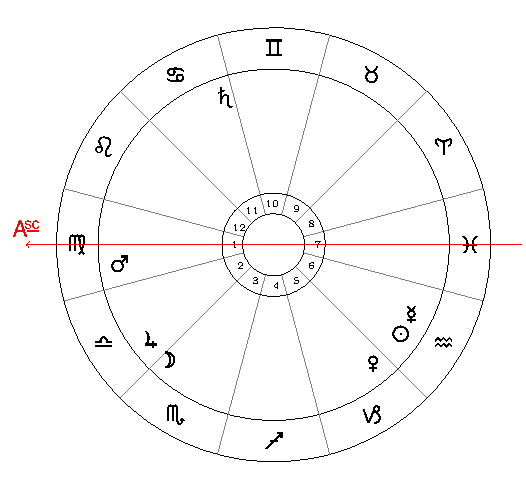
\includegraphics[width=.68\textwidth]{charts/5_09_1}
\caption{Chart 54 [V.9, GH L120,II]}
\label{fig:chart54}
\end{wrapfigure}

From \Mars\, and the Ascendant to \Jupiter\, there are 2 signs, from \Jupiter\, to the \Moon, 2 signs, and from \Venus\, to \Mercury\, and the \Sun, 2 signs. So the years, 2, 4, 6, 8, 10 apply to them.

Then from \Mars\, to the \Moon\, are 3 signs, from \Saturn\, to \Mars\, 3, from the \Moon\, to \Venus\, 3. So the years 3, 6, 9, 12, 15 apply to them.

Then we count 4 from \Saturn\, to \Jupiter, 4 from \Jupiter\, to \Venus, and 4 from the \Moon\, to the \Sun\, and \Mercury. So the years 4, 8, 12, 16 apply to them.

Then from \Mars\, and the Ascendant to \Venus\, there are 5 signs, from \Jupiter\, to the \Sun\, and \Mercury, 5, and from \Saturn\, to the \Moon, 5. So the years 5, 10, 15, 20 apply to them.

Then again from \Mars\, and the Ascendant to the \Sun\, and \Mercury\, there are 6 signs, and from the \Sun\, and \Mercury\, to \Saturn, 6. So the years 6, 12, 18, 24, 30 apply to them.

Then from \Saturn\, to \Venus\, there are 7 signs, and <from \Venus\, to \Saturn, 7.> So the years 7, 14, 21, 28, 35 apply to them.

Next from \Saturn\, to the \Sun\, and \Mercury\, there are 8 signs, and from the \Sun\, and \Mercury\, to \Mars\, and the Ascendant 8. So the years 8, 16, 24, 32, 40 belong to them.

Next from the \Sun\, and \Mercury\, to \Jupiter\, there are 9 signs, from \Venus\, to \Mars\, and the Ascendant, 9, and from the \Moon\, to \Saturn, 9. So the years 9, 18, 27, 36, 45 apply to them.

Next from the \Sun\, and \Mercury\, to the \Moon\, there are 10 signs, from \Venus\, to \Jupiter, 10, and from \Jupiter\, to \Saturn, 10. So the years 10, 20, 30, 40, 50 apply to them.

Then from \Venus\, to the \Moon\, there are 11 signs, from \Moon\, to \Mars\, and the Ascendant, 11, and
from the Ascendant and \Mars\, to \Saturn, 11. So the years 11, 22, 33, 44, 55 apply to them.

Then from the \Sun\, and \Mercury\, to \Venus\, there are 12 signs, from the \Moon\, to \Jupiter, 12, and from \Jupiter\, to \Mars\, and the Ascendant, 12. So the years 12, 24, 36, 48, 60 apply to them. One will find <the year> by continuing the enumeration as far as one wishes.

This number is powerful even when doubled because of the nature of the chart. In many nativities the number which is derived as a factor of the 12-year number seems more scientific and effective. Consequently it is necessary to note \textbf{/213P/} it <the year of the cycle> first, then divide by 12 \textbf{/224K/} and investigate the remainder <=find the number modulo 12>. If it is found to have a transmission, use it even more. If it is not so found, we will have to factor it or the number less than it. 

An example: if we are investigating year 20, we subtract 12 and investigate the remainder 8, to see if a transmission is there\footnote{If there are planets in the 8th place there is a transmission(?)}. If
none is found, we investigate the places 4 signs apart and use them just like the 8 (for this transmission will be quite influential), or we could investigate those places 2 signs apart, for the factors 8 are 2 and 4. (2x4=8, and 4x2=8) The transmissions will be influential if this is so.

Next the numbers 21 and 19 give information by their being in opposition: if we subtract 12 from 19, 7 is left; and if we multiply 3 times 7, we find 21. 

For the number 27, the <signs> 3 and 9 signs apart will be influential. 

If the year 24 is found to have a transmission, I will use it because of the factor 3. The stars which are 13, 25, or 37 signs apart stop at the same sign\footnote{The numbers 13 and 37 are prime numbers, their only factors are one and themselves. The number 25 has three factors, 1, 5 and itself; since 5 x 5 = 25 it ``stops'' at itself as well (?)}. If a star is in that sign, it will be transmitting to the <same> sign. If, when the star is there, other stars are in the next sign in order of the signs, it will transmit to them instead. 

Using the previous nativity as an example: in the 13th and 25th
years\footnote{Both years equate to the first house: 13 - 12 = 1, 25 - (2 x 12) = 1.}, \Mars\, transmits to \Jupiter\, and \Jupiter\, to the \Moon. If no stars are found in the next sign, the stars transmit the year to themselves. 

Now each number seems to be most scientifically used when its own natural interrelationships are taken into account. Therefore in distributing the circles we will most appropriately first use 12, because of the 12 signs, then 7 because of the 7 stars. If no transmission of 12 signs is found where it must happen from these\footnote{If there is no transmission found when distributing the `circle' (signs) giving 1 year to each then distribute based on the 7 planets giving 1 year to each (?) So, using the example chart, would you start from \Mars, giving him one year, year 2 to \Jupiter\, year 3 to the \Moon, etc(?)}…

But I must add this most scientific explanation: it is necessary to make the \mn{vital sector} vital sector run from every star to the degree-position of the encounter and of the ray-casting <of benefics or malefics>, and to determine the causative force of each star relative to any other star. If the Ascendant, the \Sun, or \Moon\, is considered to be the apheta, and any one of these three travels its course through the transitions of the chronocrators, arrives at the rays which are cast by benefics or malefics (or to their degree-positions), and becomes the cause of good or bad, or even brings the end sometimes—if this is so, why can the other stars not effectively act as the apheta or the ray-caster <=anaereta>? Or shall we assign the rulership of the vital
sector to these three alone <Ascendant \Sun\, \Moon> and ignore the rest as if they were firmly fixed and planted like <mere> signposts. <No>, every star moving in its own \textbf{/214P/} course of wind <=direction> will be productive of good or bad. I am aware of this fact since I have tested it by experience: many times, although I have found no appropriate controller, no houseruling cause, nor seen any influence from another source, great and unexpected occasions of good have arisen. At other times dangerous and fatal circumstances have ensued. I understood these occasions from the vital sector of the stars: when malefics in their degree-motions\footnote{Motion by zodiacal degree or ascensions?} come to the Ascendant, the \Sun, or the \Moon, they bring the end; when they come to MC or the “opportune”
places, they bring unemployment and upsetting or dangerous crises. (In their turn, benefics bring rank, preeminence, and profits, if the apheta of the basis of the nativity is found at the \Sun, the \Moon, or the Ascendant, and at the houseruler.)

Concerning the other types of affairs and the kinds of livelihoods, it is necessary to pay attention to the aphetic points, aspects, and ray-casting of the other stars. For how could \Saturn\, and \Mars\, not produce illness, sudden critical times, the deaths of fathers and mothers, hostility from the great, ruin of rank, degree position, at the Ascendant, the \Sun, or the \Moon\, (providing that the nativity has sufficient years)? How could they <\Saturn\, and \Mars> not bring the deaths of wives and other females, hostility from them, trouble, life-crises, rebukes, and shameful passions, when they are in the places and degrees of \Venus? How could they not bring trials and abuse because of documents, money, or religious matters, or the deaths of brothers, relatives, and slaves, when they are in the places of \Mercury? How could they not bring rank, stewardships, acquisition, childbirth, success, political ties with the great, when they are in the places of
\Jupiter?

In the same way, each star will be influential according to the power of itself and of those stars which are in conjunction or which are casting rays. If they are in operative signs or at the angles, they will be more definite and positive in their results, less so if they precede the angles. 

If a star is found to be \mn{retrograde} retrograde, we will make its vital sector run upwards <in the direction of diurnal rotation>, not in the order
of signs. Then, having determined at which point its retrograde period ends, we will examine what star is able to cast rays to that point during that chronocratorship. If it is turned away from the presence of any star or angle, \textbf{/226K/} it will cast rays from one sign to another sign which is the length of its retrograde period away, and it will be influential for good or bad.

It is necessary to calculate the motions in degrees using the books of the tables of visible motions\footnote{Not clear if he is speaking of ascensional degrees and tables, planet motion and emphemeris tables or both. For example, you could look at an emphemeris to see when a retrograde period ends but still `move' the planets by ascension degrees.}, \textbf{/215P/} because the overall basis and the sequence of chronocrators is controlled by these vital sectors. As a result of not knowing that predictions are made using many methods, and since they have devoted themselves to applying one method to every case, most men have knowledge which is nonexistent, ineffective, or careless. Those who have accurately operated with many methods and who have used a scientific system which employs methods appropriate to the nativity possess a careful grasp of the effects of causative influences. 

Just as men from all climes come to various cities, particularly to the royal city <Alexandria>, many men from all directions, but not all approaching by the same road: some arrive from afar on foot, travelling desert places and rough roads and falling into fearsome dangers; others travel the thoroughfares easily and safely; others come through storms at sea and blasts of winds, often picturing death
to themselves—all to attain their goals. No form of contest nor prize for their journey, either short or difficult, is placed before them. Rather each one attains profit, rank, or his particular goal (according to the
influence of his current chronocrator), or he becomes involved in crises and is ruined—or even loses his life. On some doom comes slowly. Others expect a swift end, but <gain> unexpected good fortune. 

Our situation is as complex: we must attend to our studies and come to the art of forecasting as if we were travelling by many roads. For many thousands of events happen to men, events which cannot be
grasped through the use of one method or star, but through the use of many. 

Knowing that twelve Places are indicative for each nativity and that very many configurations can be derived from these Places and from
the nature of the stars, we must observe the position of the angles and the interchange of the Places. Often two Places fall together in one sign, or a presumed angle really just precedes the <true> angle. This also occurs with the events indicated by the Ascendant.

\textbf{/227K/} An example: \Gemini\, in the Ascendant, MC in \Aquarius\, when calculated by degree. This X Place includes the Places relevant to action, to rank, and to children. It also includes the Places of Foreign Lands and of the God, since it is found (when calculated by sign) in the IX Place from the Ascendant, and the transmission operative from places 4 and 5 signs apart acts from it to the Ascendant, while the transmission operative from places 9 and 10 signs apart acts from the Ascendant to it. In the same way the
sign in opposition to \Aquarius\, (\Leo, which is IC) includes the Places relevant to buildings, estates, and parents, and the Places of the Goddess, brothers, and strangers; the transmission from places 3 /\textbf{216P/} and 4 signs apart acts from the Ascendant to it, while the transmission from places 10 and 11 signs apart acts from it to the Ascendant. 

Let the same calculation be made for the other signs, particularly for those of long rising time, because in those signs, MC would be sextile <to the Ascendant>. In short, if we calculate the Places and the distances between stars by degree <not just by sign>, we will not go astray\footnote{Advocating the use of whole sign places and dynamic places(?)}.

\begin{wrapfigure}[16]{R}{7cm}
\centering
\vspace{-20pt}
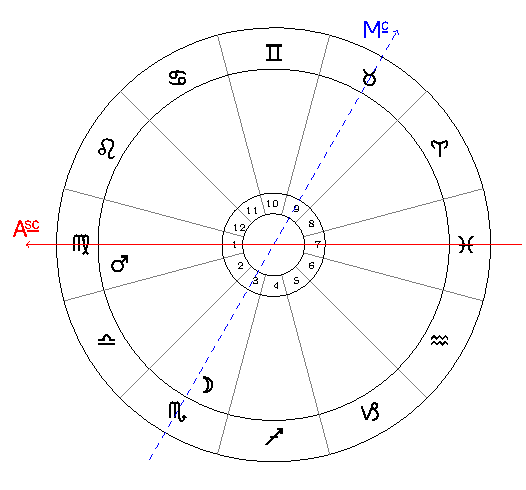
\includegraphics[width=.68\textwidth]{charts/5_09_2}
\caption{Chart 55 Partial Chart}
\label{fig:chart55}
\end{wrapfigure}

An example: \Mars, Ascendant in \Virgo, \Moon\, in \Scorpio\, at IC, MC in \Taurus. 


It is necessary to investigate the 34th year. 34 divided by 12 gives 2, with a remainder of 10. The transmission can go from the \Moon\, to \Mars, since they are both at angles <10 signs apart>, and from the Ascendant and \Mars\, to \Taurus\, (i.e. to MC)\footnote{If the places were divided based on the degrees of the angles (as in modern house systems), the IC would mark the beginning of the 4th place, the MC, the 10th.}. During this period the client worked abroad, was a friend of great men, was in mortal danger because of a woman, and suffered cuts and bleeding. Other transmissions were operative at this time, but they did not reveal the <particular> crisis.

To sum up: often opportunities for bad things arise even when the chronocrator is not under suspicion; on the other hand, great rank and profit follow even if the chronocrator does not seem to promise these
things.


\newpage